% !TEX TS-program = pdflatex
% !TEX encoding = UTF-8 Unicode

% This file is a template using the "beamer" package to create slides for a talk or presentation
% - Talk at a conference/colloquium.
% - Talk length is about 20min.
% - Style is ornate.

% MODIFIED by Jonathan Kew, 2008-07-06
% The header comments and encoding in this file were modified for inclusion with TeXworks.
% The content is otherwise unchanged from the original distributed with the beamer package.

\documentclass{beamer}


% Copyright 2004 by Till Tantau <tantau@users.sourceforge.net>.
%
% In principle, this file can be redistributed and/or modified under
% the terms of the GNU Public License, version 2.
%
% However, this file is supposed to be a template to be modified
% for your own needs. For this reason, if you use this file as a
% template and not specifically distribute it as part of a another
% package/program, I grant the extra permission to freely copy and
% modify this file as you see fit and even to delete this copyright
% notice. 
\usepackage{caption}
\usepackage{subcaption}

\mode<presentation>
{
  \usetheme{Warsaw}
  % or ...

  \setbeamercovered{transparent}
  % or whatever (possibly just delete it)
}


\usepackage[english]{babel}
\usepackage[export]{adjustbox}
% or whatever

\usepackage[font={scriptsize}]{caption}
\usepackage[utf8]{inputenc}
%\usepackage{amsmath}
% or whatever
%\usepackage[font=small]{caption}
\usepackage{graphicx}
\usepackage{times}
\usepackage[T1]{fontenc}
%\newcommand{\source}[1]{\caption*{\hfill Source: {#1}} }
% Or whatever. Note that the encoding and the font should match. If T1
% does not look nice, try deleting the line with the fontenc.


\title[Class] % (optional, use only with long paper titles)
{Classification of AGNs and Pulsars using Machine Learning techniques }

%\subtitle
%{Include Only If Paper Has a Subtitle}

\author{Aakash Bhat and Dmitry Malyshev}%(optional, use only with lots of authors)
% - Give the names in the same order as the appear in the paper.
% - Use the \inst{?} command only if the authors have different
%   affiliation.

\institute % (optional, but mostly needed)
{
 FAU Erlangen-Nurnberg
 % University of Somewhere
  %\and
 % \inst{2}%
 % Department of Theoretical Philosophy\\
 % University of Elsewhere}
% - Use the \inst command only if there are several affiliations.
% - Keep it simple, no one is interested in your street address.
}
\date{Juli 2019} % (optional, should be abbreviation of conference name)
% - Either use conference name or its abbreviation.
% - Not really informative to the audience, more for people (including
%   yourself) who are reading the slides online

\subject{Astronomy}
% This is only inserted into the PDF information catalog. Can be left
% out. 



% If you have a file called "university-logo-filename.xxx", where xxx
% is a graphic format that can be processed by latex or pdflatex,
% resp., then you can add a logo as follows:

% \pgfdeclareimage[height=0.5cm]{university-logo}{university-logo-filename}
% \logo{\pgfuseimage{university-logo}}



% Delete this, if you do not want the table of contents to pop up at
% the beginning of each subsection:
\AtBeginSubsection[]
{
  \begin{frame}<beamer>{Outline}
    \tableofcontents[currentsection,currentsubsection]
  \end{frame}
}


% If you wish to uncover everything in a step-wise fashion, uncomment
% the following command: 

%\beamerdefaultoverlayspecification{<+->}


\begin{document}

\begin{frame}
  \titlepage
\end{frame}

\begin{frame}{Table of contents}
  \tableofcontents
  % You might wish to add the option [pausesections]
\end{frame}


% Structuring a talk is a difficult task and the following structure
% may not be suitable. Here are some rules that apply for this
% solution: 

% - Exactly two or three sections (other than the summary).
% - At *most* three subsections per section.
% - Talk about 30s to 2min per frame. So there should be between about
%   15 and 30 frames, all told.

% - A conference audience is likely to know very little of what you
%   are going to talk about. So *simplify*!
% - In a 20min talk, getting the main ideas across is hard
%   enough. Leave out details, even if it means being less precise than
%   you think necessary.
% - If you omit details that are vital to the proof/implementation,
%   just say so once. Everybody will be happy with that.

\section{Introduction}

\subsection{General Idea}

\begin{frame}

  \begin{itemize}
  \item
Create machine learning algorithms capable of classifying AGNs and Pulsars
  \item
   Use 4-year Fermi LAT catalog to train and test the algorithms
  \item
Apply the algorithms on the newly released 8-year list

  \end{itemize}
\end{frame}


\subsection{Application}

\begin{frame}{Types of sources and algorithms}
 \begin{itemize}
  \item
Use the classified AGNs (BL lacs etc) and Pulsars
  \item
	Find the appropriate "features" to use
  \item
Algorithms include: Random forests, Logistic regression, Neural Networks
  \item
	Estimate performance by focusing on individual models (Number and depth of trees in forest based models, Number of layers in Neural networks)
\end{itemize}
\end{frame}

\begin{frame}{Testing and Predictions}
 \begin{itemize}
  \item
Use the classified sources from 8 year list to test algorithms
  \item
	Predict for unassociated sources in 8 year list
  \item
      Further predictions on sub-classes

\end{itemize}
\end{frame}
\section{The Data}

\subsection{AGNs and PSRs}

\begin{frame}{}
\begin{itemize}
 \item
Total of 1905 sources classified in the 4 year list
 \item
Features: Flux, uncertainty, Significant curvature, spectral index, Hardness ratios,  Galactic latitude
 \item
70\% training and 30\% testing 
 \item
$hr_{ij}=\frac{EnergyFlux_j - EnergyFlux_i}{EnergyFlux_j + EnergyFlux_i}$

\end{itemize} 

\end{frame}

\begin{frame}{}
\begin{figure}[!h]
    \centering
    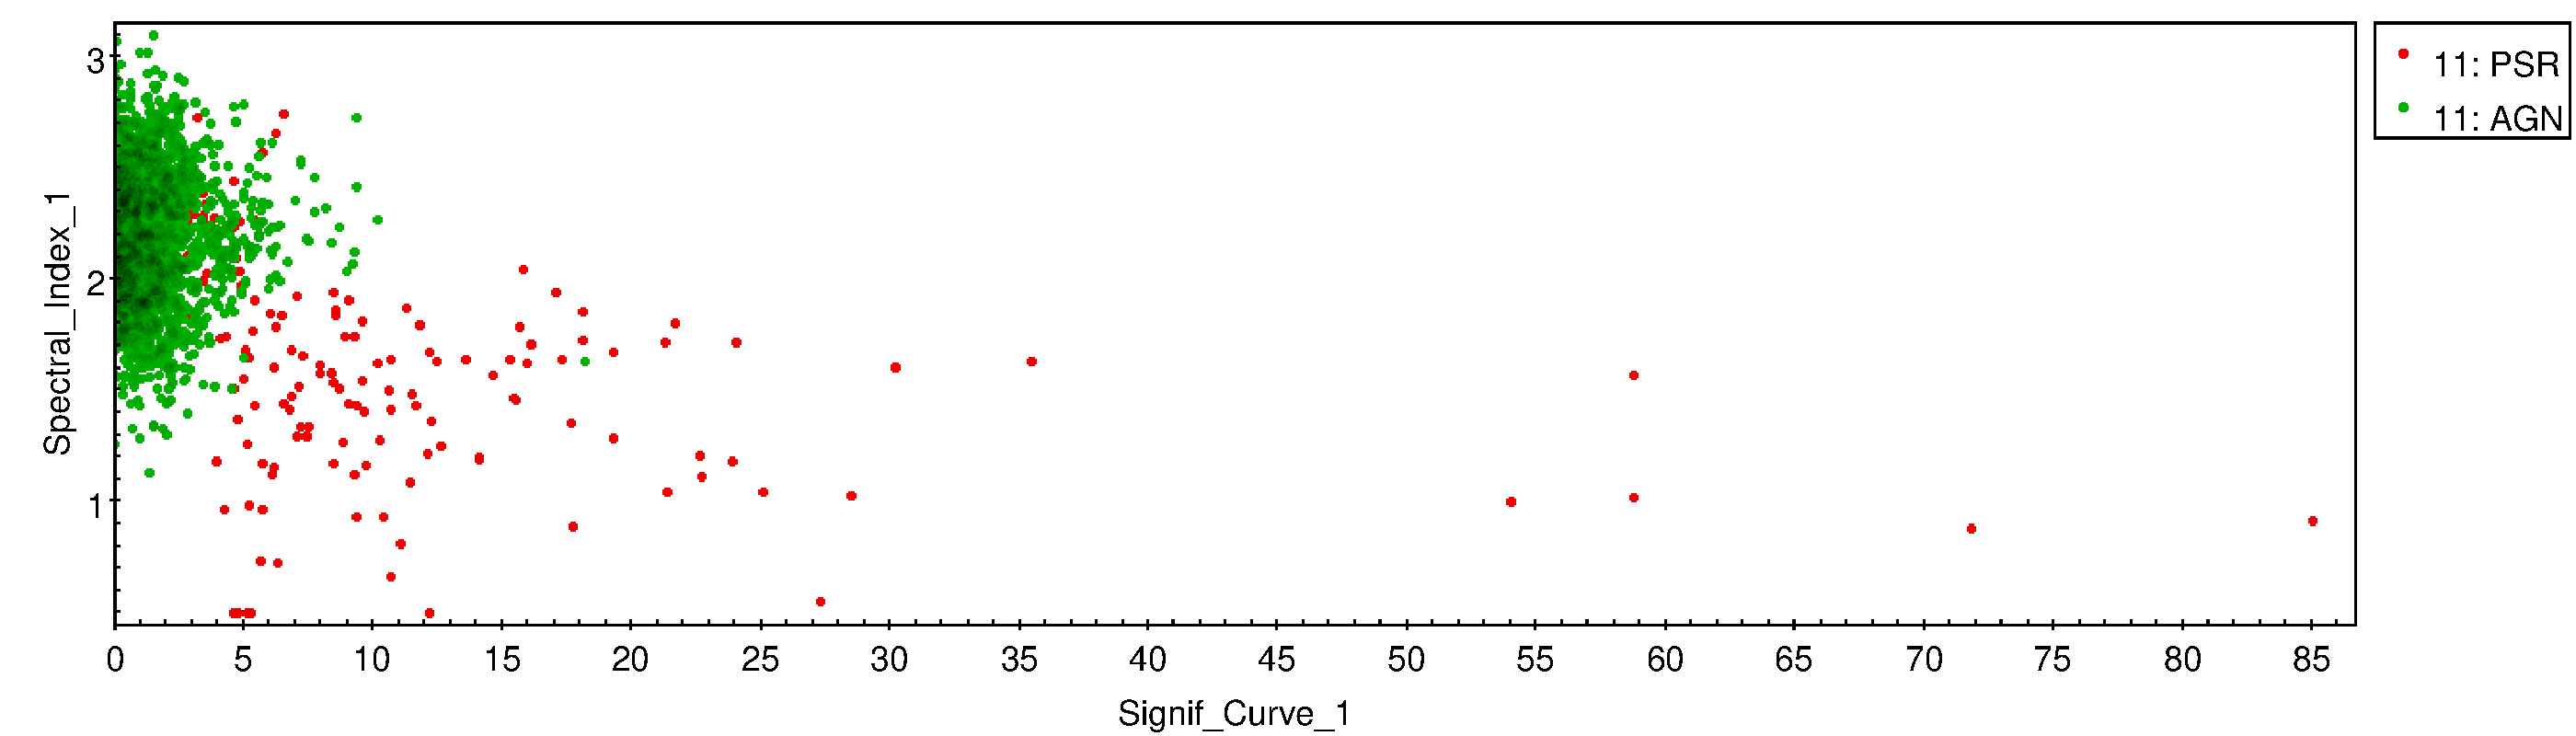
\includegraphics[height=4cm,width=11 cm]{signifcurvvsspecind}
    \caption{Motivation for classification}
    \label{fig:mot}
\end{figure}
\end{frame}

\begin{frame}{}
\begin{figure}[!h]
    \centering
    \includegraphics[height=6cm,width=11 cm]{correlation2.pdf}
    \caption{Correlation Matrix}
    \label{fig:corr}
\end{figure}
\end{frame}


\section{Algorithms}
\begin{frame}{tweaking}
\begin{figure}[!h]
    \centering
    \includegraphics[height=5cm,width=8 cm]{rf_numvsscore}
    \caption{Score vs. Number of trees}
    \label{fig:mot}
\end{figure}
\end{frame}
\begin{frame}{}
\begin{figure}[!h]
    \centering
    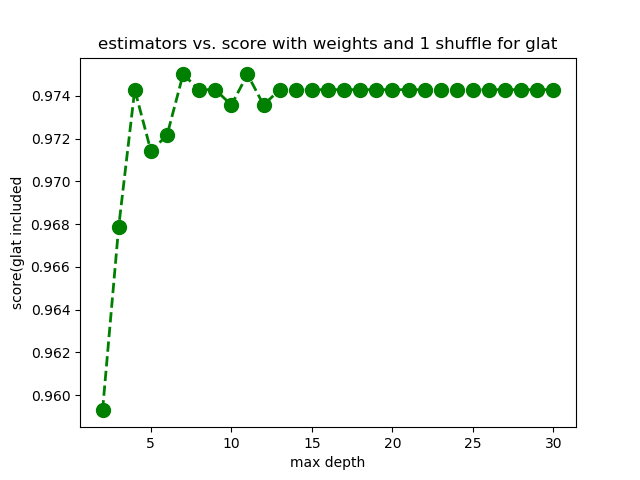
\includegraphics[height=6cm,width=8cm]{Rf_maxdepth_oobscore_glat}
    \caption{Score vs. Maximum depth of trees}
    \label{fig:mot}
\end{figure}
\end{frame}
\begin{frame}
\begin{table}[!h]
    \centering
    
    \begin{tabular}{|c|c|}
    \hline
    Algorithm&Percentage\\
     \hline
    Random Forest & 97.03\\
    \hline %\midrule   -> aakash do you mean this?
    Extra Trees Classifier& 97.03 \\
    \hline
    Gradient Boost & 96.79\\
    \hline %\midrule   -> aakash do you mean this?
    Ada Boost& 97.53 \\
    \hline %\midrule   -> aakash do you mean this?
    Logistic Regression& 95.06 \\
    \hline
     
    \end{tabular}

    \caption{Scores for training data}
    \label{tab:my_label}
\end{table}{}
\end{frame}

\begin{frame}
\begin{table}[!h]
    \tiny
    \centering
    \renewcommand{\tabcolsep}{1mm}
\renewcommand{\arraystretch}{1.5}

    \begin{tabular}{|c|c|c|c|c|c|c|c|c|c|c|c|}
    \hline
    Algorithm &Fluxden & Uncertainity & Index&Signifcurv&Var&GLAT&hr12&hr23&hr34&hr45\\
    \hline
    Random Forest& 0. &        0. &        0.106 &0.287 &0.1006& 0.062& 0.048& 0.058& 0.0605& 0.275  \\
    \hline
    Extra Trees & 0.       &  0. &        0.152 &0.340 &0.086& 0.077& 0.064 &0.059& 0.0747 &0.144\\
    \hline %\midrule   -> aakash do you mean this?
    Gradient Boost& 0.      &   0.   &      0.021 & 0.528 &0.308  &0.020& 0.006& 0.034 &0.027 &0.053 \\
    \hline %\midrule   -> aakash do you mean this?
    Ada Boost& 0. &  0. &  0.12& 0.16& 0.12 &0.26& 0.1 & 0.06& 0.04 &0.14 \\
    \hline
     
    \end{tabular}

    \caption{Importance of Features}
    \label{tab:my_labe2l}
\end{table}{}
\end{frame}

\begin{frame}
\begin{figure}[!h]
    \centering
    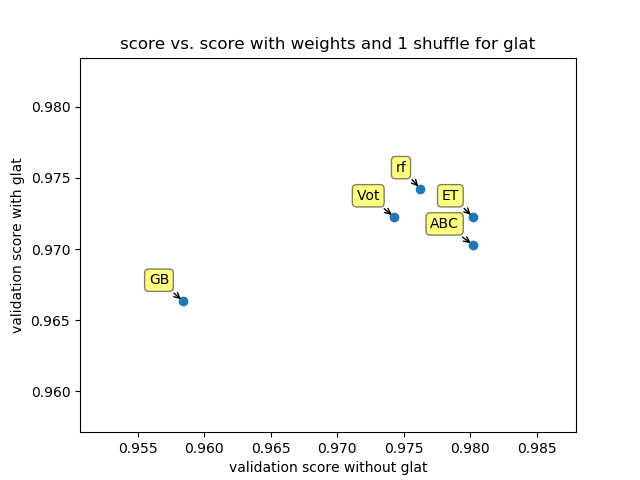
\includegraphics[height=5cm,width=7 cm]{classifiers_max_depth_15}
    \caption{Scores with and without GLAT}
    \label{fig:mot}
\end{figure}

\end{frame}

\begin{frame}{Testing Data}
\begin{figure}[!h]
    \centering
    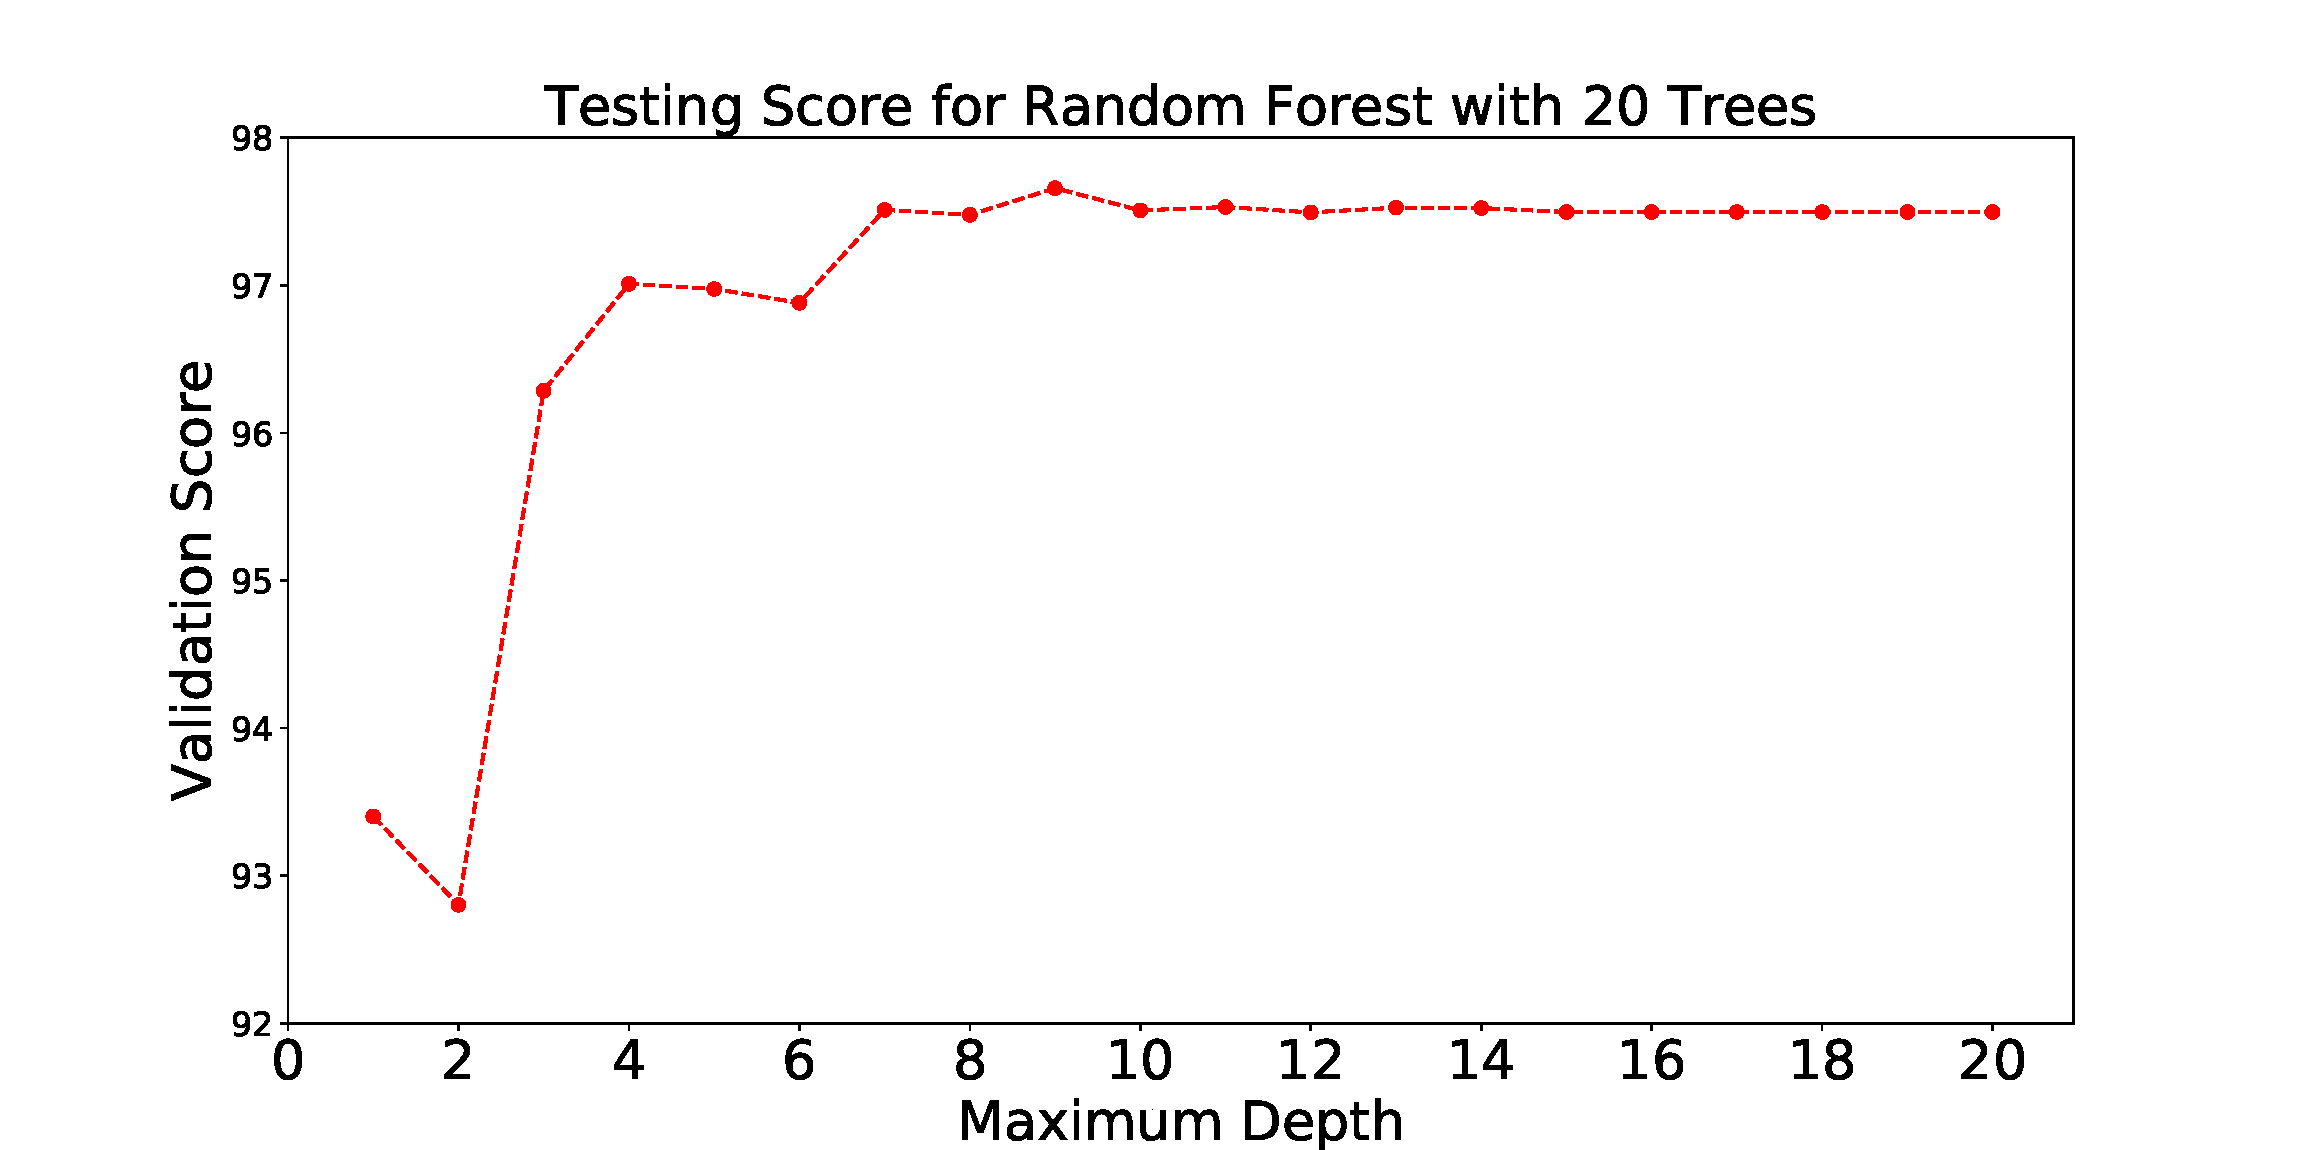
\includegraphics[height=5cm,width=8 cm]{depthvsscore_rf_10seeds_20trees}
    \caption{Dependence of scores on maximum depth of Random Forests}
    \label{fig:mot5}
\end{figure}

\end{frame}

\begin{frame}
\begin{figure}[!h]
    \centering
    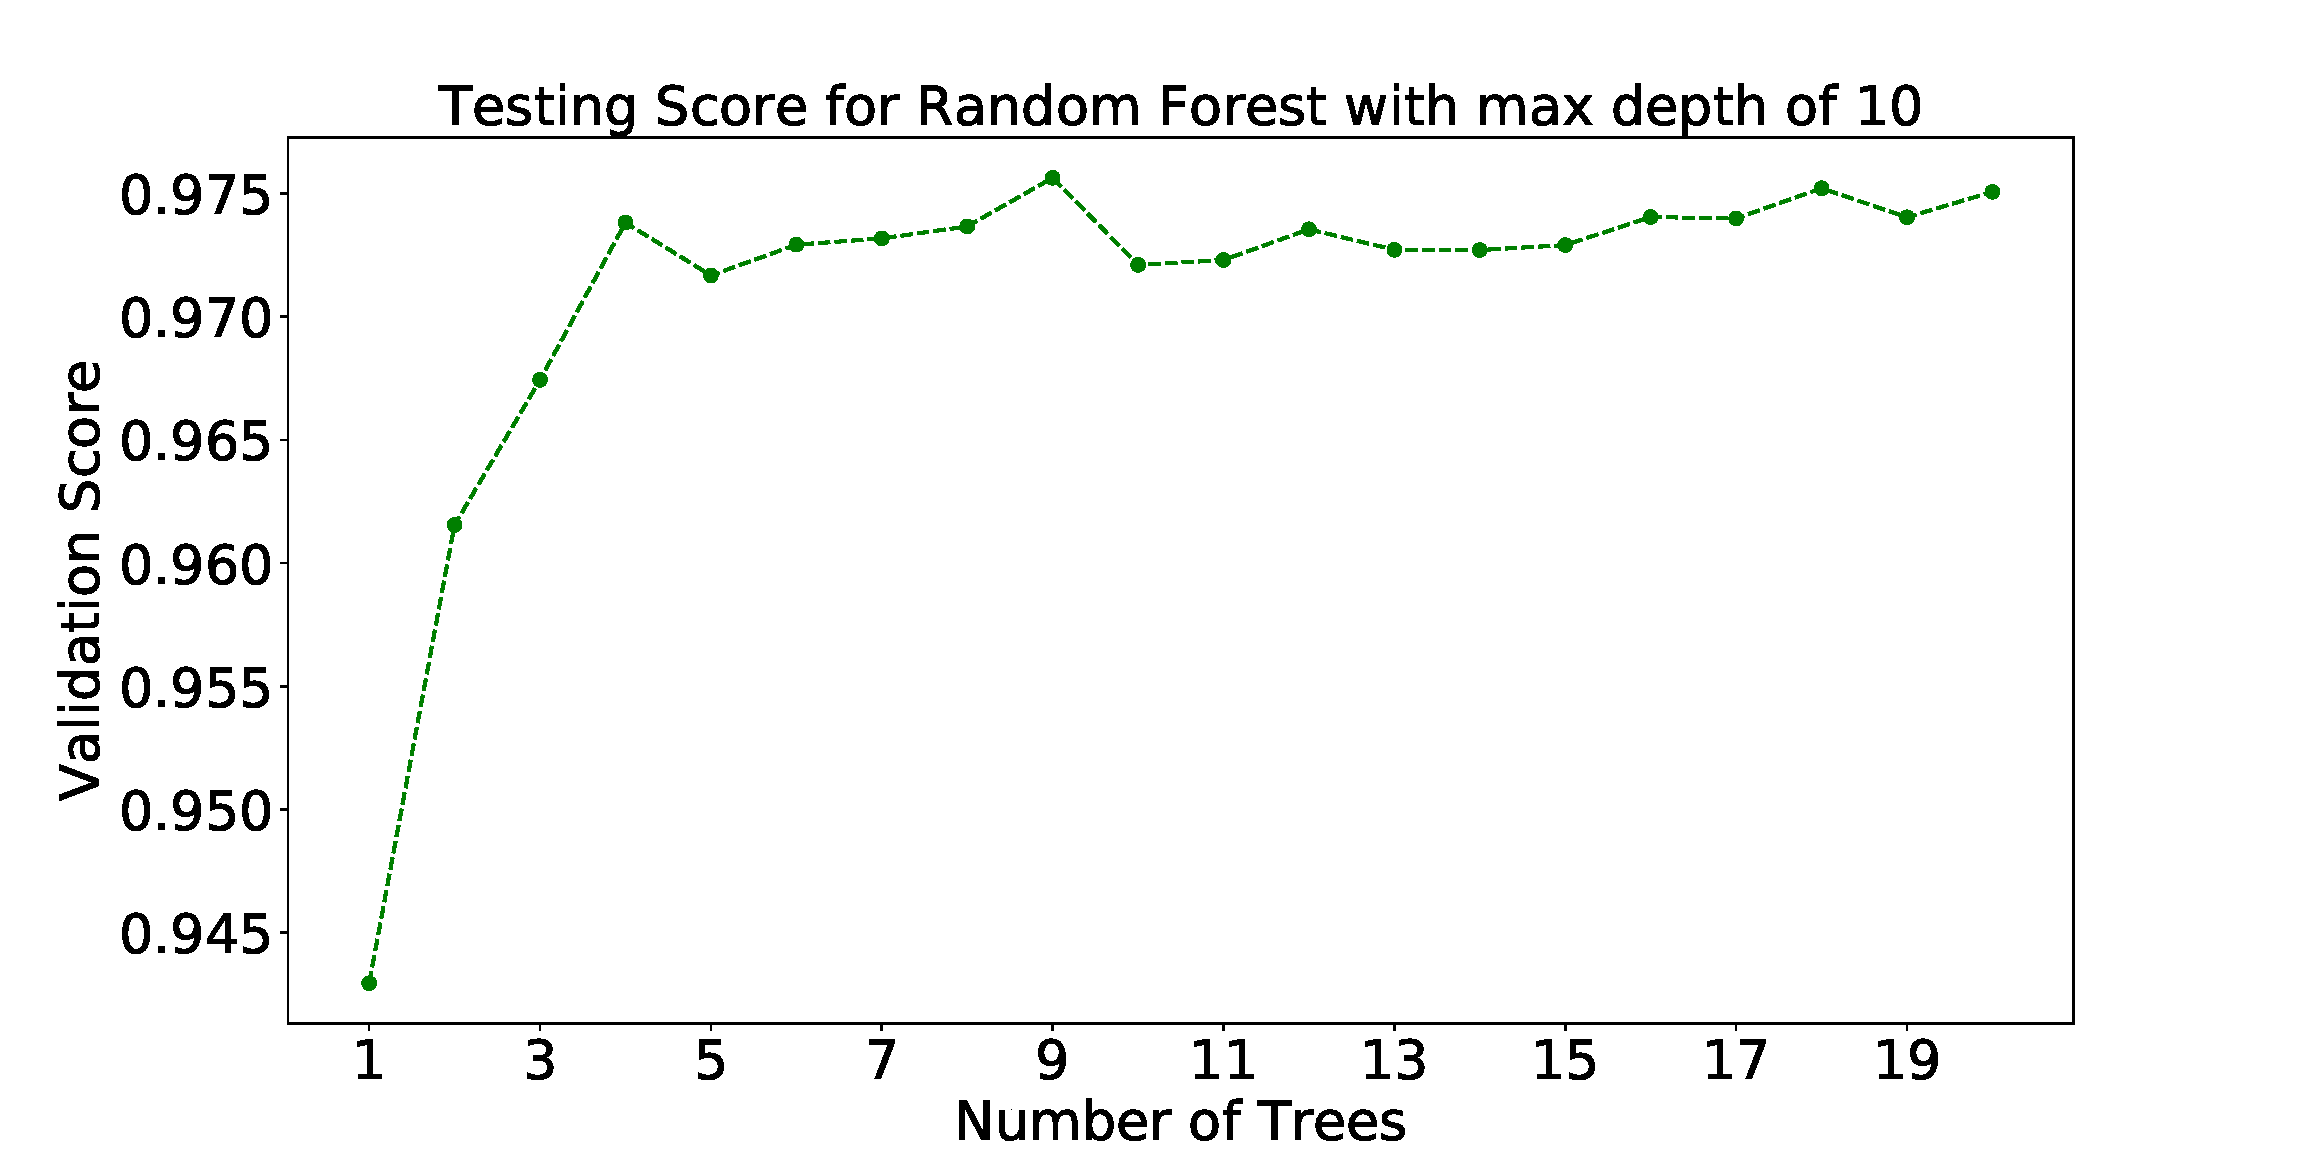
\includegraphics[height=5cm,width=8 cm]{treesvsscore_RF_10seeds_10maxdepth}
    \caption{Dependence of scores on number of trees for Random Forests}
    \label{fig:mot4}
\end{figure}
Similar Studies for two other Classifiers 
\end{frame}

\begin{frame}{Classification Domains}
%Using Classification Domains to get a closer look at the algorithm for bias and variance purposes
\begin{figure}[!h]
\centering
	\begin{subfigure}[b]{\linewidth}
    		\centering
    		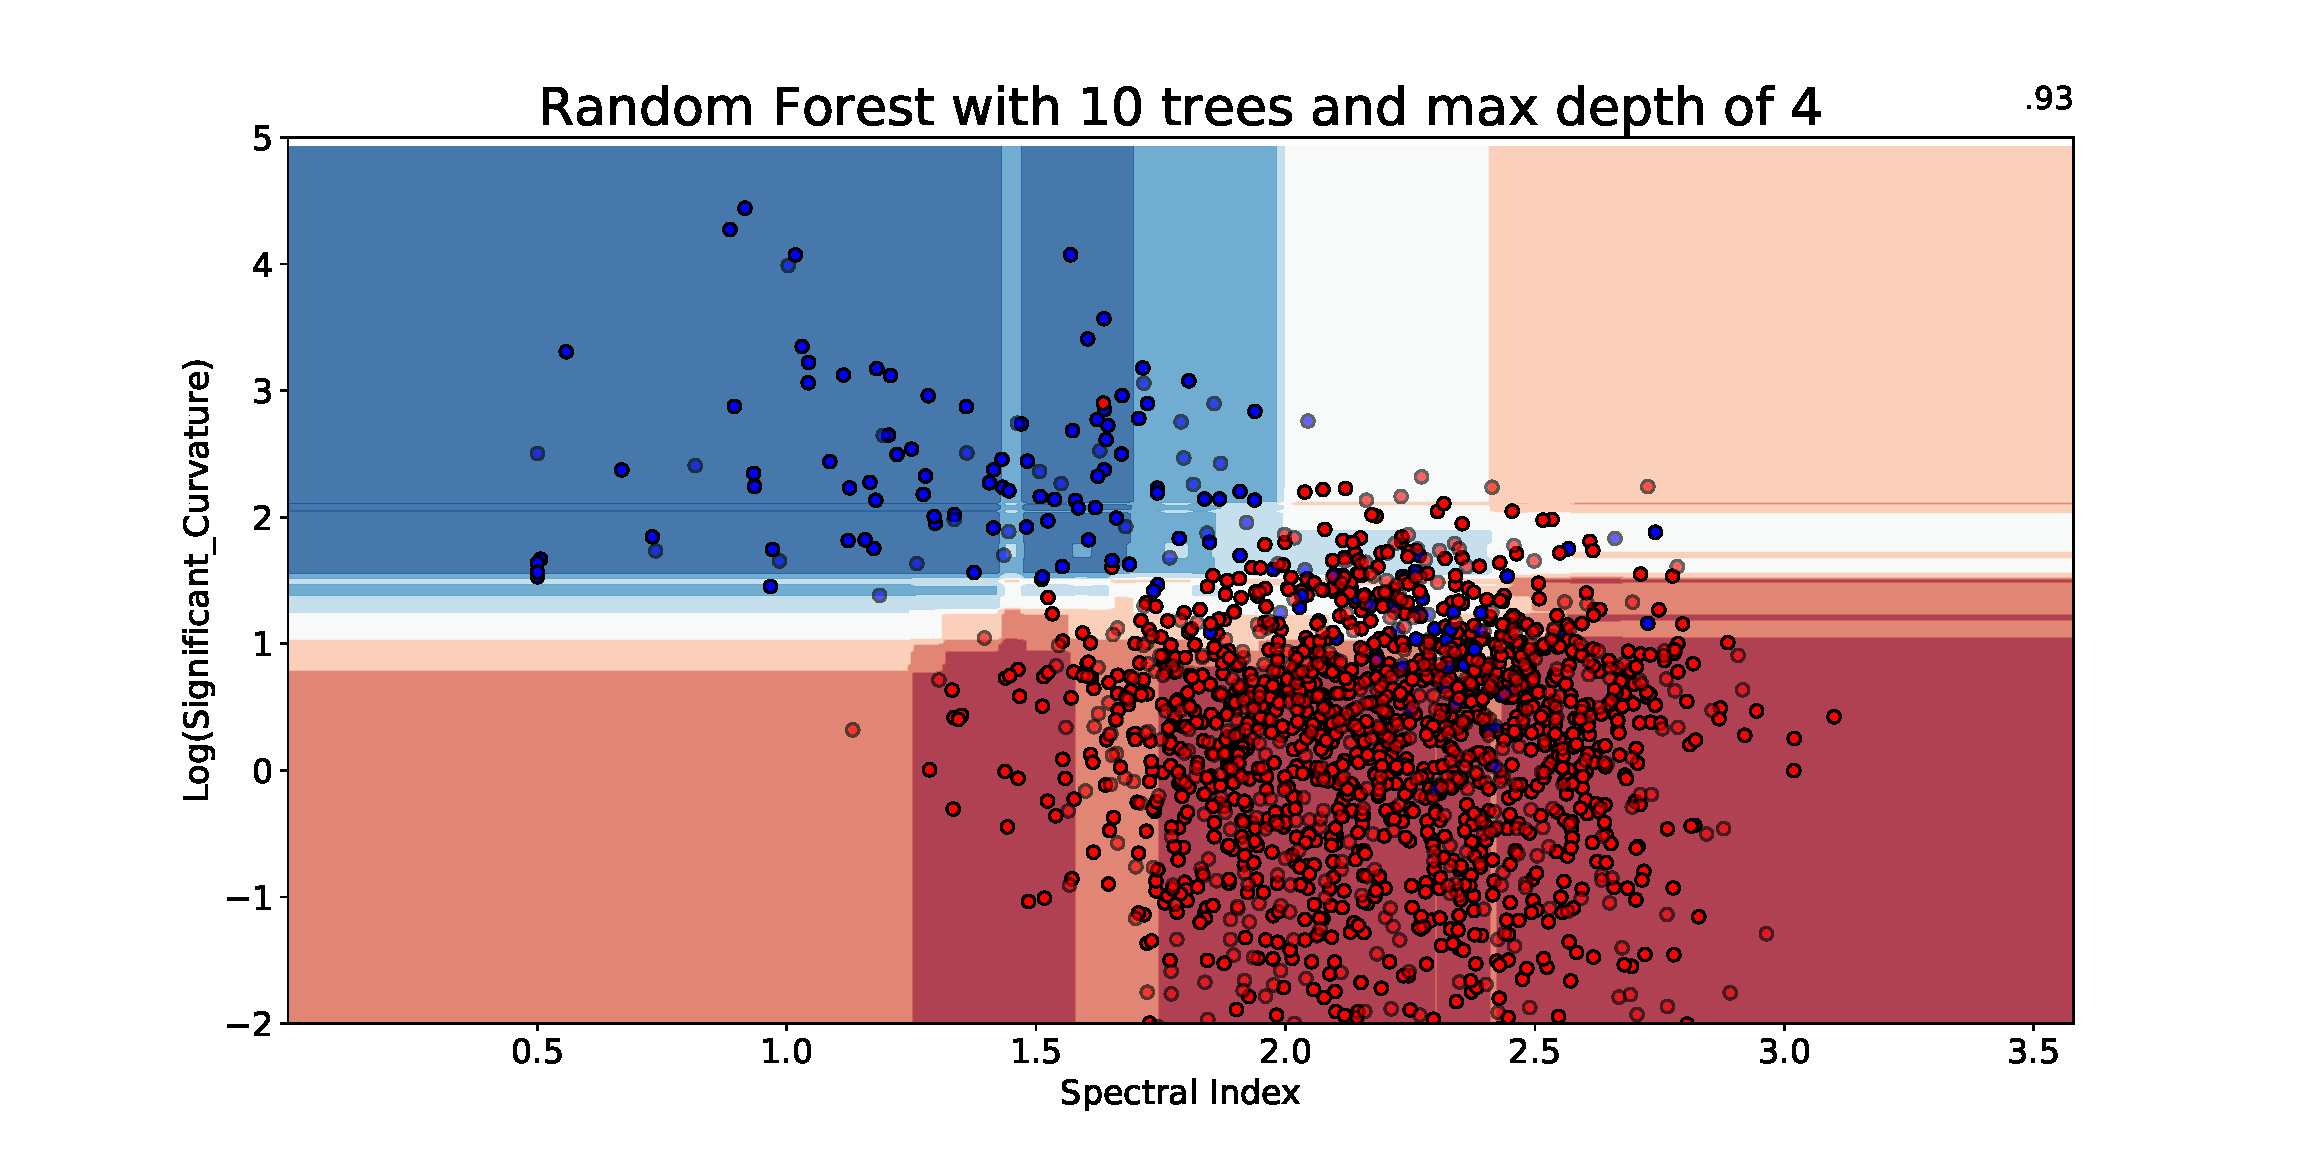
\includegraphics[width=0.5\textwidth]{classification_domains(rf_10trees_4maxdepth_weightbalanced_oobscoretrue)}
    		\caption{Classification Domains for RF with 10 trees and 4 Max Depth}
    		\label{fig:mot3}
	\end{subfigure}
	
	\begin{subfigure}[b]{\linewidth}
    		\centering
    		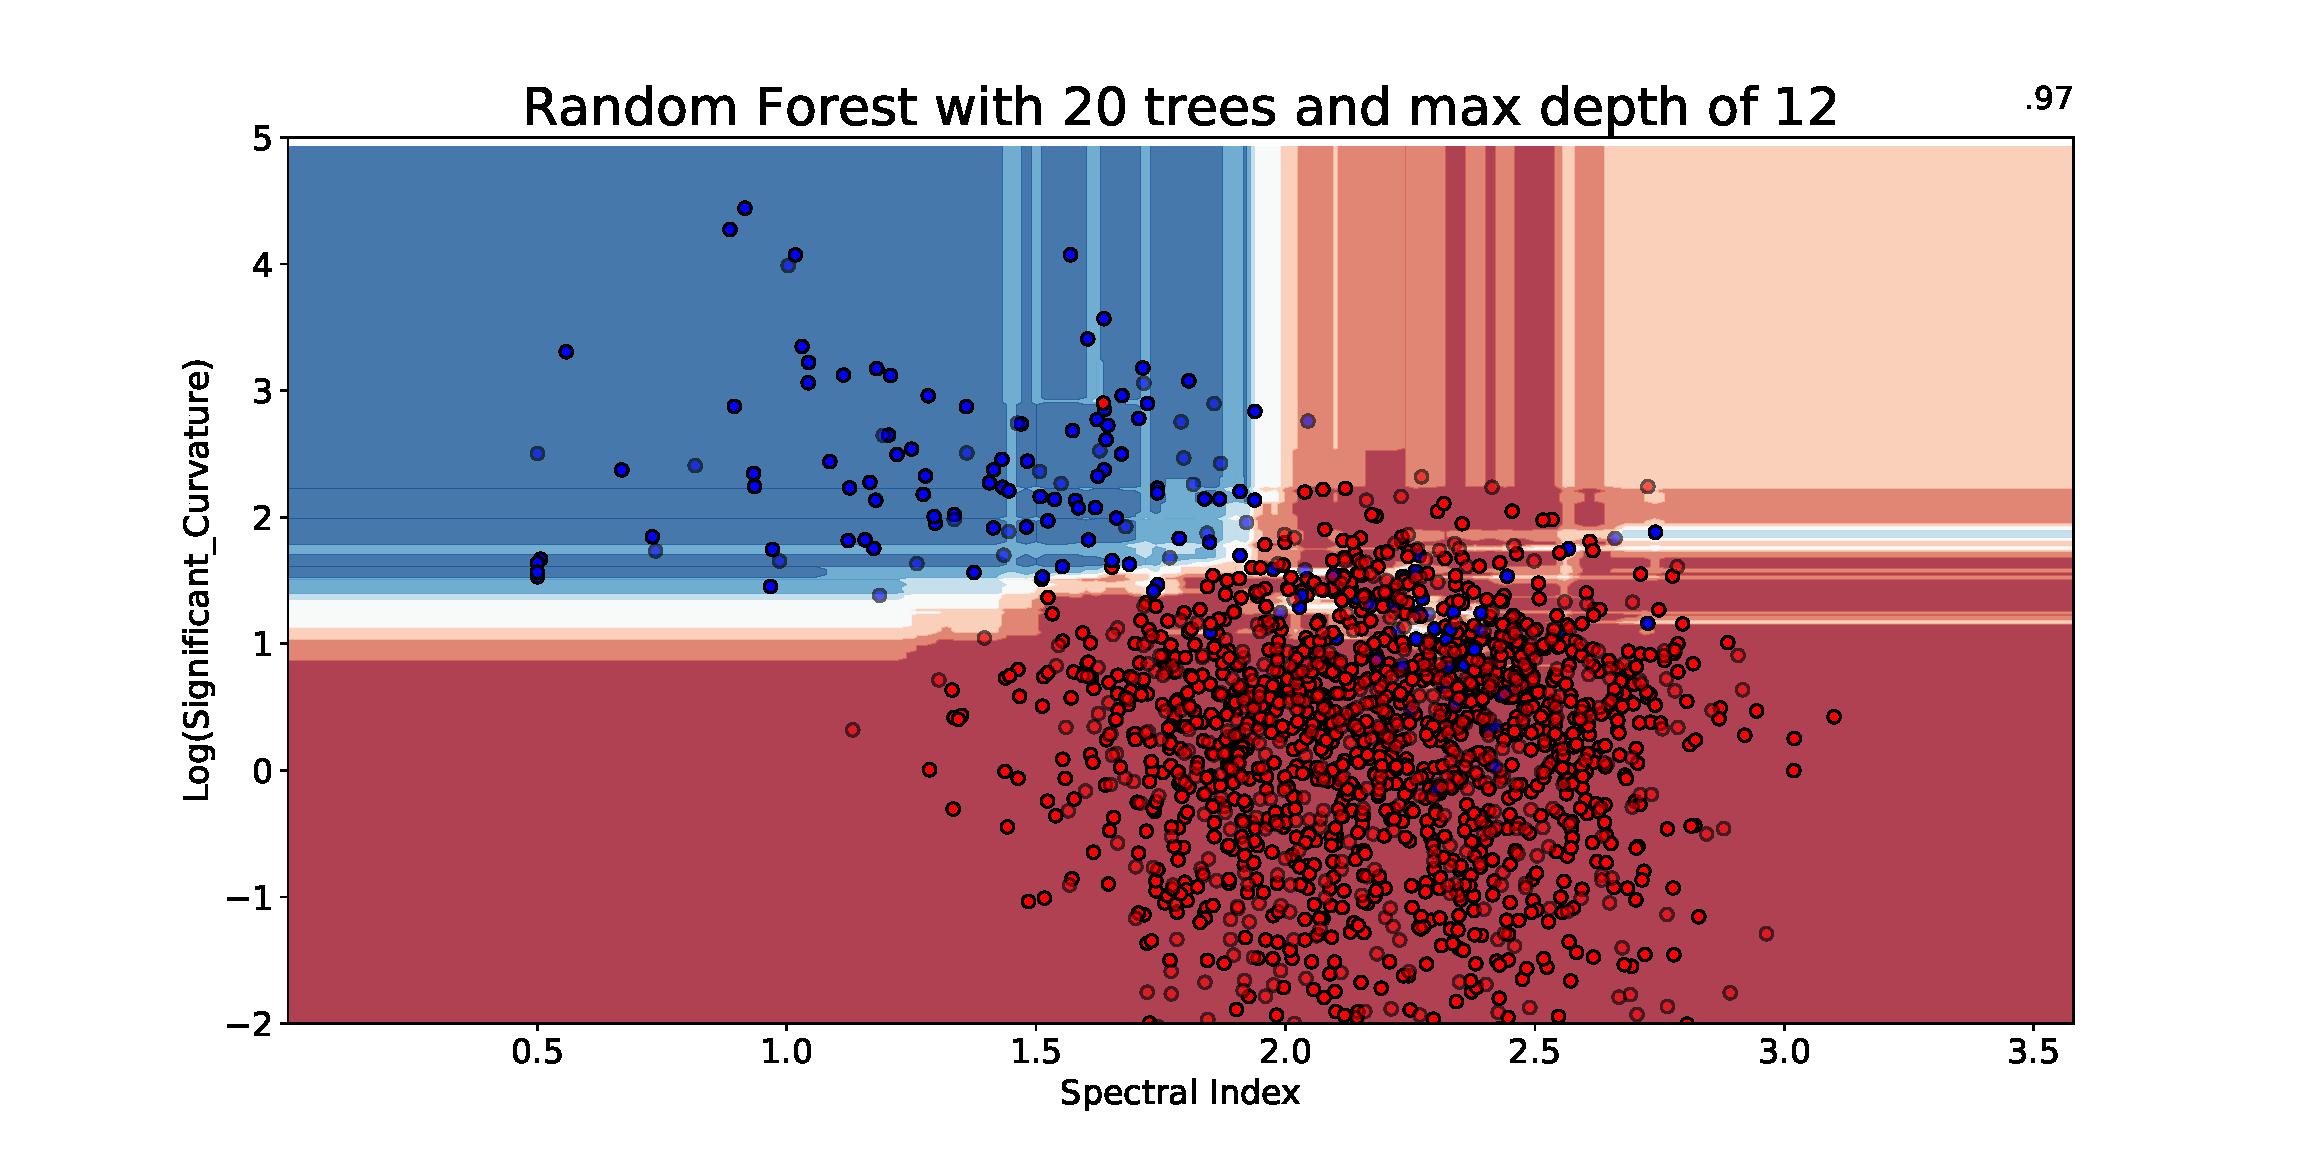
\includegraphics[width=0.5\textwidth]{classification_domains(rf_20trees_12maxdepth_weightbalanced_oobscoretrue)}
    		\caption{Classification Domains for RF with 20 trees and 12 Max Depth}
    		\label{fig:mot2}
	\end{subfigure}
\end{figure}
%Similar Studies for two other Classifiers 
\end{frame}


\section{Actual Data}
\begin{frame}
\begin{itemize}
\item Testing on unassociated data with classes from FL8Y
\end{itemize}
\begin{table}[!h]
    \centering
    
    \begin{tabular}{|c|c|}
    \hline
    Algorithm&Percentage\\
     \hline
    Random Forest & 95.45\\
    \hline %\midrule   -> aakash do you mean this?
    Extra Trees Classifier& 96.5 \\
    \hline
    Gradient Boost & 96.15\\
    \hline %\midrule   -> aakash do you mean this?
    Ada Boost& 96.15 \\
    \hline %\midrule   -> aakash do you mean this?
    Logistic Regression& 88.11 \\
    \hline
     
    \end{tabular}

    \caption{Scores for actual testing data}
    \label{tab:my_label}
\end{table}{}
\end{frame}
\begin{frame}{Neural Networks}

  % Keep the summary *very short*.
  \begin{itemize}
  \item
    Neural Networks with 1-2 hidden layers
  \item
    Hyperbolic Tan as activation function and Sigmoid as the final layer
  \item
   Give accuracy above 90\% (Max accuracy of 98\%).
   
  \end{itemize}
  
\end{frame}


\begin{frame}
\begin{itemize}
\item Predicting on Unassociated Data
\end{itemize}
\begin{table}[!h]
    \centering
    
    \begin{tabular}{|c|c|c|}
    \hline
    Algorithm&Accuracy& Expected Pulsars (1056 sources)\\
     \hline
    RF (50,12) & 98.30&148\\
    \hline %\midrule   -> aakash do you mean this?
    BDT(50,15)& 96.86&184 \\
    \hline
    NN(20 N, 200 E) &98.09& 213\\
    \hline
     
    \end{tabular}

    \caption{Performance and Prediction of three types of classifiers}
    \label{tab:my_label}
\end{table}{}
\end{frame}
\begin{frame}{Future Work}

  % Keep the summary *very short*.
  \begin{itemize}
 % \item
   % Optimize all the algorithms
  \item
    Predict for fl8y unassociated sources and match with other catalogs
  \item
  Predict for further sub-classes (BLLACS and FSRQs, yng and ms PSR)
   
  \end{itemize}
  
\end{frame}




\end{document}


